\documentclass{article}
\usepackage[utf8]{inputenc}
%packages used
\usepackage[left=3cm, right=3cm, top=3cm]{geometry}
\usepackage[utf8]{inputenc}
\usepackage{amsmath, amssymb}
\usepackage{graphicx}
\usepackage{hyperref}
\usepackage{enumerate}
\usepackage[hang,flushmargin]{footmisc}
\usepackage{amsfonts}
\usepackage{amsthm}
\usepackage{xcolor}
\usepackage{centernot}
\usepackage{multicol}
\usepackage{color}
\usepackage{verbatim}
\usepackage{caption}
\usepackage{subcaption}
\usepackage{epsfig}
\usepackage{tikz-cd}
\graphicspath{ {./images/} }


\graphicspath{ {./images/} }

\newtheorem{theorem}{Theorem}
\newtheorem{lemma}{Lemma}
\newtheorem{corollary}{Corollary}
\newtheorem{definition}{Definition}

%newly defined commands
\renewcommand{\today}{}
\newcommand{\abs}[1]{\left| #1\right|}
\newcommand{\Lap}[1]{\mathcal{L}\left\{#1\right\}}
\newcommand{\solution}[1]{
    \color{red}\begin{quote}Solution:\quad 
    \color{black} #1
    \end{quote}\color{black}
}
\newcommand{\ba}{\backslash}
\newcommand{\Ber}{\hbox{Ber}}
\newcommand{\p}[1]{\mathbb{P}\left(#1\right)}
\newcommand{\e}[1]{\mathbb{E}(#1)}
\newcommand{\Po}[1]{\hbox{Po}(#1)}
\newcommand{\var}[1]{\hbox{Var}(#1)}
\newcommand{\Z}{\mathbb{Z}}
\newcommand{\R}{\mathbb{R}}
\newcommand{\Q}{\mathbb{Q}}
\newcommand{\N}{\mathbb{N}}
\newcommand{\floor}[1]{\left\lfloor #1\right\rfloor}
\newcommand{\C}{\mathbb{C}}
\DeclareMathOperator{\Diam}{diam}
\newcommand{\diam}[1]{\Diam\left(#1\right)}
\DeclareMathOperator{\nul}{Null}
\newcommand{\Null}[1]{\nul\left(#1\right)}
\DeclareMathOperator{\Dimension}{dim}
\newcommand{\Dim}[1]{\Dimension\left(#1\right)}
\newcommand{\threevec}[3]{\left[\begin{array}{r} #1 \\ #2 \\ #3\end{array}\right]}
\newcommand{\fourvec}[4]{\left[\begin{array}{r} #1 \\ #2 \\ #3\\#4\end{array}\right]}
\DeclareMathOperator{\Rank}{rank}
\newcommand{\rank}[1]{\Rank\left(#1\right)}
\DeclareMathOperator{\Nullity}{nullity}
\newcommand{\nullity}[1]{\Nullity\left(#1\right)}
\DeclareMathOperator{\Sp}{Span}
\renewcommand{\sp}[1]{\Sp\left\{#1\right\}}
\DeclareMathOperator{\col}{Col}
\newcommand{\Col}[1]{\col\left(#1\right)}
    

 

\title{Markov Chains}
\author{Akshath Jain \& Deepayan Patra}
\date{December 2018}

\usepackage{natbib}
\usepackage{graphicx}

\begin{document}

\maketitle

\section{Overview}
<Comments> 
add comment in main that say adjList is initial input of links given
State that damping factor d can be changed based on case being considered
Could you my name to top of code, change the date, fix purpose to new project
Review things i wrote once make sure they make sense lol
</Comments>


Describe Page-Rank, what it does, its relation to Markov Chains
Describe purpose of Page-Rank
Expand to other applications of markov chain models:
See this source:
%https://projecteuclid.org/download/pdfview_1/euclid.ps/1208958281
Cite this source (thx):
%http://mathworld.wolfram.com/MarkovChain.html
Just do some of the below:

For the Kids: Snakes and Ladders
%https://scipython.com/book/chapter-6-numpy/additional-problems/analysing-snakes-and-ladders-as-a-markov-chain/
High-School Example: Populations and Predator-Prey Relationships
%http://acadpubl.eu/jsi/2017-117-11-14/articles/11/35.pdf

Markov-Chain Monte Carlo Methods
%https://towardsdatascience.com/a-zero-math-introduction-to-markov-chain-monte-carlo-methods-dcba889e0c50

Chemical Reaction Mechanisms
%3.3 in Euclid

Differential Equations
%5.1 in Euclid

\section{A Brief History of Markov Chains and Page-Rank}
Might want to combine this section with previous.

\section{Referenced Definitions and Theorems}
    This section outlines major definitions and theorems referenced throughout the rest of the paper.
    \subsection{Definitions}
    
    \begin{definition}{Web Graph$^{[]}$ SHUM}
    
    \noindent
    \textup{A web graph is directed graph representation of interconnected states such that individual states are represented as nodes and possible ordered changes in state are represented as directed edges from one node to the next according to a probabilistic model.}
    
    \end{definition}
    
    \begin{definition}{Transition/Stochastic Matrix$^{[]}$ LAY ROUSSEAU SHUM WOLFRAMSTOCHASTIC}
    
    \noindent
    \textup{An $n \times n$ stochastic matrix $P$ contains entries representing the probability that a change in state occurs from one state to another. Specifically, the $P_{ij}$ entry of the matrix, the entry in the $i^\text{th}$ row and the $j^\text{th}$ column, determines the probability that an input will change to state $i$ given that the input starts at state $j$. In other words, ``$p_{ij}$ is the conditional probability that we are on the $i$-th page at step $n+1$ given that we were on the $j$-th page at step $n$'', with $p_{ij}$ equivalent to the $P_{ij}$ entry.$^{[]}$ ROUSSEAU Thus, each term in matrix is greater than or equal to 0, and in a normal transition matrix, the sum of the terms in each column add to 1 as the rows of the matrix construct the sample space for the possible change of states (and the probabilities over a sample space sum to 1).}
    
    \end{definition}
    
    \begin{definition}{Steady-State/Equilibrium Vector$^{[]}$ LAY TANASE}
    
    \noindent
    \textup{The steady-state or equilibrium vector is the vector such that $$P \Vec{x} = \Vec{x}$$ which is the eigenvector corresponding to an eigenvalue of $1$ for the regular stochastic matrix $P$. This vector $\Vec{x}$ represents the convergence of the probabilities upon repeated multiplications (tending towards infinity) by $P$ given any initial state $x_0$.}
    
    \end{definition}
    
    \begin{definition}{Dangling Node$^{[]}$ SHUM}
    
    \noindent
    \textup{A dangling node exists in a web-graph when the matrix representation of the graph has a column of all $0$s. This implies that the node does not allow a following state as no outgoing links exist.}
    
    \end{definition}
    
    \begin{definition}{Altered Transition Matrix$^{[]}$ SHUM}
    
    \noindent
    \textup{In the case that a dangling node exists, it is not initially possible to construct a regular stochastic matrix from the given probabilities. To instead construct a representation of the probabilities, we replace the column of $0$s with a column of the form
    $$\begin{bmatrix} \frac{1}{N} \\ \frac{1}{N} \\ \vdots \\ \frac{1}{N} \end{bmatrix}$$ where $N$ is the number of nodes in the graph. This representation defines that the following node will be picked randomly from the $N$ possible nodes and is referred to as an altered transition matrix.}
    
    \end{definition}
    
    \begin{definition}{Irreducible Graph$^{[]}$ SHUM}
    \noindent
    \textup{An irreducible graph contains distinct nodes that can pairwise be reached through traversal of the web-graph. Specifically, ``a graph is called irreducible if for any pair of distinct nodes, we can start from one of them, follow  the links in the web graph, and arrive at the other node, and vice versa.''$^{[]}$ (Shum)}
    
    \end{definition}
    
    \begin{definition}{Reducible Graph$^{[]}$ SHUM}

    \noindent
    \textup{According to Shum, a reducible graph is any graph that is ``not irreducible'' as defined above.$^{[]}$ A reducible graph forces the issue that the probabilities of arriving at a specific node are altered by the creation of a cycle within a subset of the web graph, preventing traversal to previous nodes despite their nonzero reachability.}
    
    \end{definition}
    
    \begin{definition}{Damping Factor$^{[]}$ SHUM ROUSSEAU TANASE}
    
    \noindent
    \textup{A positive constant damping factor $\beta$ chosen from $[0,1]$ is utilized for reducible graphs such that we replace the transition matrix $P$ with $ \widetilde{P}$ defining $$\widetilde{P} = \beta P + \frac{1-\beta}{n} \begin{bmatrix} 1 & 1 & \ldots & 1 \\ 1 & 1 & \ldots & 1 \\ \vdots & \vdots & \ddots & \vdots \\ 1 & 1 & \ldots & 1 \end{bmatrix}$$ where we multiply the $n \times n$ matrix of ones by the factor $\frac{1-\beta}{n}$, following Shum's definition (which is equivalent to, but expressed differently than Rousseau's and Tanase and Radu's representations).$^{[]}$ Rousseau expands on the explanation of reducible graphs as characterized by multiple characteristic polynomial roots of $\det{(\lambda I - A)} = 0$ such that $\lambda = 1$ or possessing ``other eigenvalues with modulus equal to 1''.$^{[]}$}
    
    \end{definition}
    
    \begin{definition}{Markov Chain$^{[]}$ ROUSSEAU WOLFRAMMARKOVCHAIN}
    
    \noindent
    \textup{A Markov chain, or a Markov chain process, is the iterative method of constructing a sequence of independent future state prediction data given initial input in the form of an $n$-term state vector $\Vec{x}_0$ and an $n \times n$ stochastic matrix $P$. Each prediction $\Vec{x}_{n+1}$, given $\Vec{x}_n$, is found through the matrix multiplication $A\Vec{x}_n$. Given a stochastic matrix, it is possible to create an altered or dampened stochastic matrix such that the adjusted matrix is regular.}
    \end{definition}
    
    \subsection{Theorems}
    \begin{theorem}{Perron-Frobenius Theorem$^{[]}$ TANASE}
    
    \noindent
    \textup{The Perron-Frobenius Theorem states that given a positive, column stochastic matrix $M$, the following three properties are satisfied:
    \begin{enumerate}
        \item 1 is an eigenvalue of multiplicity one for $M$.
        \item 1 is the largest eigenvalue; all the other eigenvalues have absolute value smaller than 1.
        \item The eigenvectors corresponding to the eigenvalue 1 have either only positive entries or only negative entries. In particular, for the eigenvalue 1, there exists a unique eigenvector with the sum of its entries equal to 1.
    \end{enumerate}
    as stated in Tanase and Radu's article.$^{[]}$}
    \end{theorem}
    
    \begin{theorem}{Power Method Convergence Theorem$^{[]}$ TANASE}
    
    \noindent
    \textup{The Power Method Convergence Theorem states that given a positive, column stochastic $n \times n$ matrix $M$, we denote $\Vec{v}^*$ as its probabilistic eigenvector corresponding to the eigenvalue 1. If we then take $\Vec{z}$ as a column vector with all entries equal to $\frac{1}{n}$, the sequence $\Vec{z}, M\Vec{z}, \ldots, M^k\Vec{z}$ converges to the vector $\Vec{v}^*$. The above definition was stated in Tanase and Radu's article.$^{[]}$ TANASE AND RADU}
    \end{theorem}
    
\section{Page-Rank Algorithm}
    This section describes the basis for the stochastic model characterized by standard Page-Rank algorithms. In addition, the material in this section describes our implementation of these techniques, encapsulated in our function definition $rank(ranks)$, which takes in as input a list of links emanating from each node represented as a 2-dimensional list, and outputs a single, ordered list of rankings. This algorithm will focus largely on the computation and construction of the Markov chain algorithm for Page-Rank. For a more probabilistic approach refer to Rousseau's consideration of conditional probabilities and their effects.$^{[]}$
    
    \subsection{Adjacency Matrix Construction and Dangling Nodes}
    Given an adjacency list, effectively an array with a list of connected nodes, we must construct a transition matrix to represent the web graph that the links define. In a simple Page-Rank algorithm, given a set of directed edges emanating from a single node, we define the probability of choosing any one of the emanating edges to be equal to the probability of choosing any other emanating edge. Therefore, for a basic case, we guarantee that the sum of the entries in any column equals 1 and that all the entries are non-negative. Thus, following Shum's algorithm example, we define an $n \times n$ matrix $P$ with entries in row $i$ and column $j$ as
    \[ P_{ij} =
    \begin{cases} 
      \frac{1}{C(j)} & \text{if there is a link from $j$ to $i$} \\
      0 & \text{in all other cases}
   \end{cases}
    \]
    where we define $C(j)$ to be the number of total outgoing edges from node $j$.$^{[]}$ However, we come upon an issue in the case of a dangling node. If a dangling node exists in an adjacency list, it is impossible to create a normal stochastic matrix without alteration, as a column of 0s does not allow for the formation of a normal stochastic matrix as the sum of the elements in the column never equals 1. Thus, again following Shum's example, in the case that we come across columns of 0s in our transition matrix $P$ representation, we replace the column of 0s with a column of the form $\begin{bmatrix} \frac{1}{n} \\ \frac{1}{n} \\ \vdots \\ \frac{1}{n} \end{bmatrix}$ so as to define that a random node will be picked after reaching a node with no emanating edges. We define this matrix to have entries of the form
    \[ P_{ij} =
    \begin{cases} 
      \frac{1}{C(j)} & \text{if there is a link from $j$ to $i$} \\
      \frac{1}{n} & \text{if there are no emanating links from node $j$} \\
      0 & \text{in all other cases}
   \end{cases}
    \]
    with $C(j)$ and $n$ as defined previously.
    
    \noindent
    Now, let us consider the implementation of this algorithmic idea in our code. First, we must initialize the size of the matrix to be $n \times n$, where $n$ is the number of nodes. We access this by taking the length of the input vector $ranks$, which has a list of connected nodes for every node, so it has $n$ elements. Now, we case on whether each node is a dangling node or not. If the node is dangling, we set each element in the column to have probability $\frac{1}{n}$. Otherwise, we construct each element of the matrix to have probability $\frac{1}{C(j)}$ where $C(j)$ is the number of elements that one node is connected to. From this, we use the numpy matrix function to construct the matrix given these values as entries for future compatability with numpy.
    
    \begin{center}
        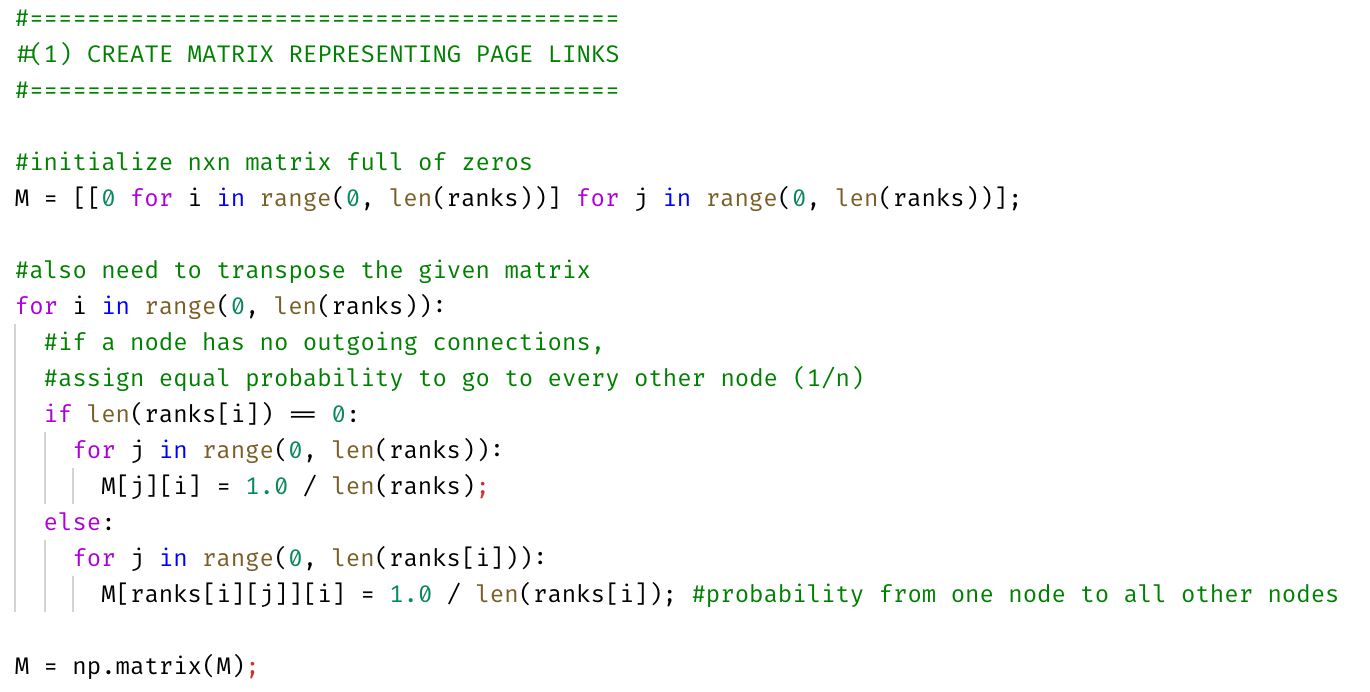
\includegraphics[scale=.6]{snip1}
    \end{center}
    
    
    \subsection{General Solution}
   
    Our generic solution then uses the Power Method Convergence Theorem to compute a close approximation to the steady-state vector that defines the ranks. As repeated multiplications by the matrix $P$ to an $n$-valued vector with terms equal to $1$ approaches an eigenvector for $\lambda = 1$, we see that a steady-state vector is approached, which is our goal. This resultant steady-state vector then defines the output rankings based on its elements.
    
    \noindent
    In code, this process is written as a loop iterating through repeated multiplications and terminating when equality is achieved, or after 1000 iterations of the loop are completed, which, as shown above, is likely to be effective for sparse matrices, as these matrices quickly converge on multiplication by a defining vector, as Tanase and Radu note.$^{[]}$
    \begin{center}
        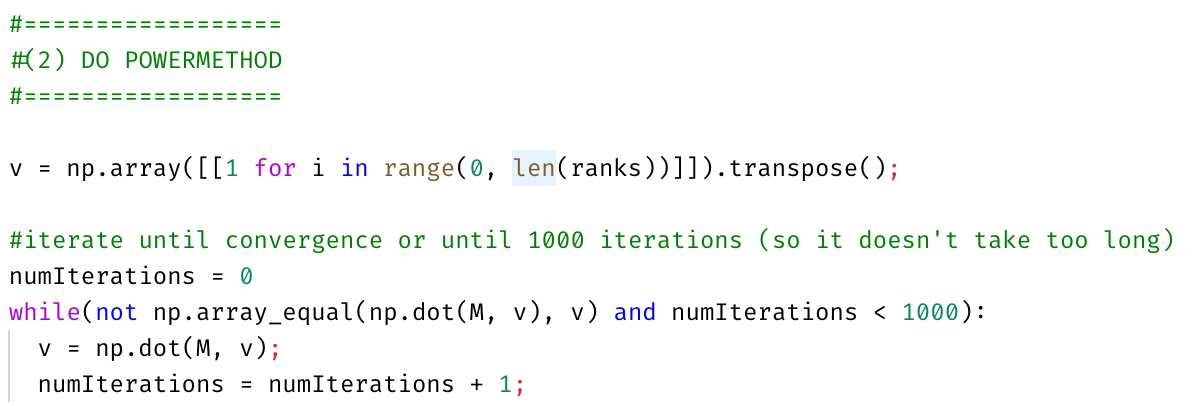
\includegraphics[scale=.6]{snip2}
    \end{center}
    Following this process, we clean our resultant vector such that the indices (and thus, nodes) are ranked in descending order, with the highest ranked node occurring first in the output vector and the lowest ranked node occurring last. Finally, we return the resulting output, our ranked list of nodes.
    
    \begin{center}
        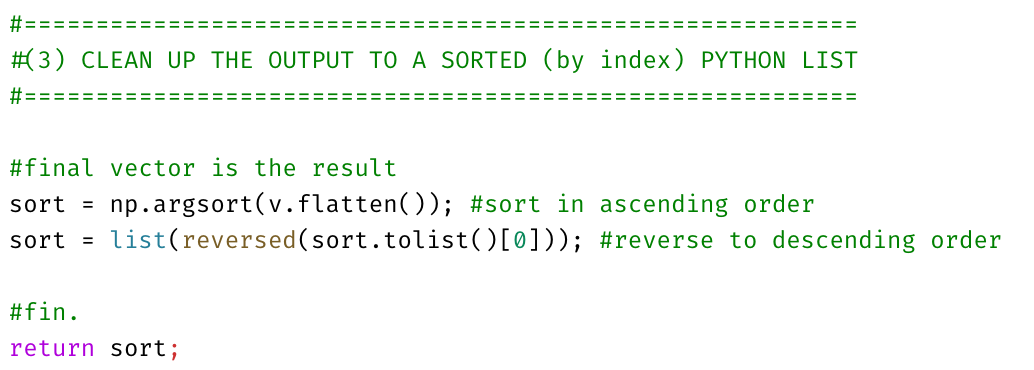
\includegraphics[scale=.6]{snip3}
    \end{center}
    
    \subsection{Damping Factors}
    In the case that our stochastic matrix $P$ is reducible, we must add an additional step to ensure continued reachability for initial nodes. We characterize this by calculating a secondary positive stochastic matrix. To do so, we utilize a damping constant $\beta$ set between $[0,1]$ as a coefficient regarding our matrix multiplication as follows: 
    $$
    M = \beta P + \frac{1-\beta}{n} \begin{bmatrix} 1 & 1 & \ldots & 1 \\ 1 & 1 & \ldots & 1 \\ \vdots & \vdots & \ddots & \vdots \\ 1 & 1 & \ldots & 1 \end{bmatrix}
    $$
    This also solves issues regarding repeated characteristic polynomial roots for $\lambda = 1$ or the possibility of the presence of multiple eigenvalues with modulus equal to 1, as Rousseau notes.$^{[]}$ We may also use this technique of damping in general, not just on reducible graphs to incorporate randomness into the probabilistic model.$^{[]}$ TANASE and RADU
    
    \noindent
    In our algorithm, we follow this process exactly, defining an all-ones matrix, a damping factor, and then redefining our matrix $M$ with the damping factor specified. From this, we proceed to the general solution as defined previously.
    \begin{center}
        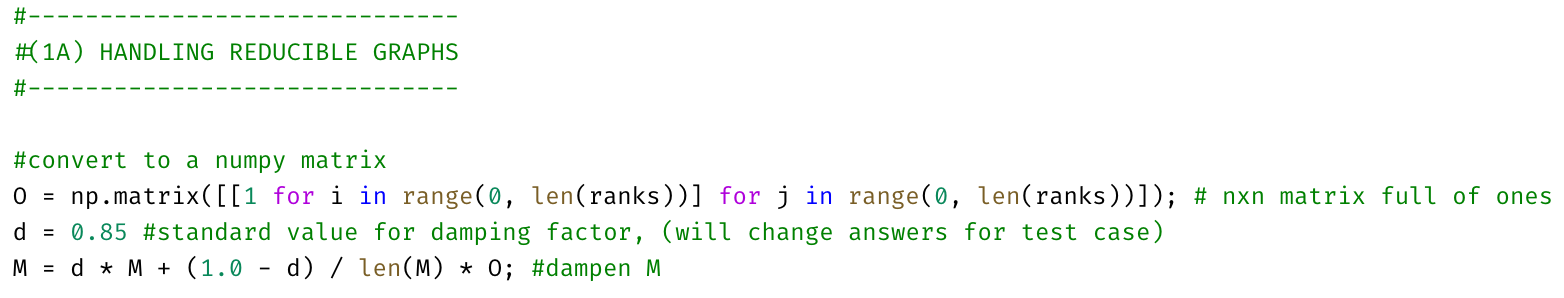
\includegraphics[scale=.5]{snip1A}
    \end{center}
    
\section{Working Examples}
    Let us consider a subset of working examples and defining behavior for the Markov chain model implemented in the previous section. The following examples will touch on some of the major points defined, first calculating the expected result, and then describing intermediate and returned results from the algorithm.
    
    \begin{enumerate}
        \item Let us consider the web graph with a damping factor of 1: 
        $$
        \begin{tikzcd}[column sep=scriptsize]
            A \arrow[dr] \arrow[rr]{}
            & & B \arrow[ll] \\
            & C \arrow[ur] \arrow[ul]
        \end{tikzcd}
        $$
        
        We input the adjacency list of connected edges of the form $\text{adjList} = [[1, 2],[0],[0, 1]]$ into our algorithm, with 0 (and index 0) corresponding to node $A$, 1 (and index 1) corresponding to node $B$, 2 (and index 2) corresponding to node $C$. The algorithm output will be described following the expected result by computation.
        
        Considering the computation by hand, from this representation, we may construct the adjacency matrix $P$ as follows:
        \begin{align*}
            P = \begin{bmatrix} 0 & 1 & .5 \\ .5 & 0 & .5 \\ .5 & 0 & 0 \end{bmatrix}
        \end{align*}
        
        By calculation, a resulting eigenvector with a column sum equal to 1 for $\lambda = 1$ is $$\vec{r} = \begin{bmatrix} r(A) \\ r(B) \\ r(C) \end{bmatrix} = \begin{bmatrix} .444 \\ .333 \\ .222 \end{bmatrix}$$
        Thus, the expected output is a ranking $A > B > C$ based on the eigenvector values.
        
        Now, returning to our algorithm, intermediately, in constructing an eigenvector in our algorithm, we observe that $$\vec{v}  = \begin{bmatrix} 1.33333333 \\ 1 \\ 0.66666667 \end{bmatrix}$$
        
        Now, observe that 
        \begin{align*}
            \frac{1}{1.33333333 + 1 + 0.66666667}(\vec{v}) = \begin{bmatrix} .444 \\ .333 \\ .222  \end{bmatrix} = \begin{bmatrix} r(A) \\ r(B) \\ r(C)  \end{bmatrix}
        \end{align*}
        
        Indeed, as expected, our algorithm returns as output $[0, 1, 2]$, meaning that $A$ has the highest rank, $B$ has the middle rank, $C$ has the lowest rank. Thus, our output matches the expected value of the calculation.
        
        \item Let us consider the following web graph with a damping factor of 1: 
        $$
        \begin{tikzcd}
            A \arrow[r] \arrow[d]
            & B \arrow[l] \\
            C 
            & D \arrow[l] \arrow[u]
        \end{tikzcd}
        $$
        
        We input the adjacency list of connected edges of the form $\text{adjList} = [[1, 2],[0],[],[1, 2]]$ into our algorithm, with 0 (and index 0) corresponding to node $A$, 1 (and index 1) corresponding to node $B$, 2 (and index 2) corresponding to node $C$, and 3 (and index 3) corresponding to node $D$. The algorithm output will be described following the expected result by computation.
        
        Considering the computation by hand, from this representation, we may construct the adjacency matrix $P$ as follows:
        \begin{align*}
            P = \begin{bmatrix} 0 & 1 & 0 & 0 \\ .5 & 0 & 0 & .5 \\ .5 & 0 & 0 & .5 \\  0 & 0 & 0 & 0\end{bmatrix}
        \end{align*}
        It is easily observable that the adjacency matrix $P$ has a dangling node, as represented by the column of 0s. Thus, we construct the altered transition matrix:
        \begin{align*}
            \widetilde{P} = \begin{bmatrix} 0 & 1 & .25 & 0 \\ .5 & 0 & .25 & .5 \\ .5 & 0 & .25 & .5 \\  0 & 0 & .25 & 0\end{bmatrix}
        \end{align*}
        By calculation, a resulting eigenvector with a column sum equal to 1 for $\lambda = 1$ is $$\vec{r} = \begin{bmatrix} r(A) \\ r(B) \\ r(C) \\ r(D) \end{bmatrix} = \begin{bmatrix} .357 \\ .286 \\ .286 \\.071 \end{bmatrix}$$
        Thus, the expected output is $A > B \geq C > D$, with $B$ and $C$ possibly switched in the output ordering based on their equivalent value.
        
        Now, returning to our algorithm, intermediately, in constructing an eigenvector in our algorithm, we observe that $$\vec{v}  = \begin{bmatrix} 1.42857143 \\ 1.14285714 \\ 1.14285714 \\ 0.28571429 \end{bmatrix}$$
        
        Now, observe that 
        \begin{align*}
            \frac{1}{1.42857143 + 1.14285714 + 1.14285714 + 0.28571429}(\vec{v}) = \begin{bmatrix} .357 \\ .286 \\ .286 \\.071 \end{bmatrix} = \begin{bmatrix} r(A) \\ r(C) \\ r(B) \\ r(D) \end{bmatrix}
        \end{align*}
        
        Indeed, as expected, our algorithm returns as output $[0, 2, 1, 3]$, meaning that $A$ has the highest rank, $C$ has the second highest rank, $B$ has the second lowest rank, and that $D$ has the lowest rank. Thus, our output matches the expected value apart from the ordering of $B$ and $C$, which is accounted for and noted in the calculation above.
    \end{enumerate}

    \noindent
    The final two examples will explore the algorithmic outputs given a larger subset of sample data, and its match with expected values provided beforehand. 
    
    \begin{enumerate}
        \item Let us consider the input of our adjacency list to be $[[1, 5], [2, 5], [1, 3, 5], [4], [1, 5], [2, 6], [0, 1]]$. We will consider this case with a damping factor of 1 and observe the output and compare with the expected output given in the test case. The algorithm output is $[5, 2, 1, 6, 4, 3, 0]$ which does not immediately seem to $[5, 2, 1, 6, 3, 4, 0]$; however, in observing the intermediate value for $\vec{v}$ in the algorithm, it is evident that with a damping factor of 1, nodes 3 and 4 have the same ranking value, so their order is interchangeable.
        
        \item Let us consider the input of our adjacency list to be $[[1,3,4],[0,2,4],[3,6],[2,4,6],[5,8], [4,6,8],$ $[0,7,9],[0,6,8],[2,9],[0,2,8]]$. We will consider this case, first with a damping factor of 1, and then with a damping factor of $.85$ and observe the outputs and compare with the expected outputs given in the test case. Indeed, the algorithm output $[2, 6, 8, 0, 3, 9, 4, 5, 7, 1]$ matches $[2, 6, 8, 0, 3, 9, 4, 5, 7, 1]$ for a damping factor of $1$, and the algorithm output $[2, 6, 8, 0, 4, 3, 9, 5, 7, 1]$ matches $[2, 6, 8, 0, 4, 3, 9, 5, 7, 1]$ with a damping factor of $.85$.
    \end{enumerate}
\section{Conclusion}




\bibliographystyle{plain}
\bibliography{references}
\begin{thebibliography}{4}

%http://mathworld.wolfram.com/MarkovChain.html
%https://projecteuclid.org/download/pdfview_1/euclid.ps/1208958281

\bibitem{lay}
Lay, D. C., Lay, S. R., \& McDonald, J. (2016). \textit{Linear algebra and its applications}. Boston: Pearson.

\bibitem{rousseau}
Rousseau, C. (2017, February 7). How Google works: Markov chains and eigenvalues. \textit{Klein Project Blog}. \texttt{http://blog.kleinproject.org/?p=280}. Accessed 13 December 2018.

\bibitem{shum}
Shum, K. (2013). \textit{Notes on Page Rank Algorithm} (tech.). \textit{Notes on Page Rank Algorithm.} \texttt{http://home.ie.cuhk.edu.hk/\~{}wkshum/papers/pagerank.pdf}. Accessed 13 December 2018.

\bibitem{stochasticmatrix}
\textit{Stochastic Matrix}. Wolfram MathWorld. \texttt{http://mathworld.wolfram.com/StochasticMatrix.html}. Accessed 13 December 2018.

\bibitem{tanase}Tanase, R., \& Radu, R. (2009). Lecture \#3: PageRank Algorithm - The Mathematics of Google Search. 
\textit{Cornell University: College of Arts and Sciences}. Cornell University. \texttt{http://pi.math.cornell.edu/\~{}mec/Winter2009/RalucaRemus/Lecture3/lecture3.html}. Accessed 13 December 2018.

\end{thebibliography}





\end{document}
